\documentclass[11pt, oneside]{book}

%%%%%%%%%%%%%%Include Packages%%%%%%%%%%%%%%%%%%%%%%%%%%
\usepackage{xcolor}
\usepackage{mathtools}
\usepackage[a4paper, total={6in, 8in}, margin=1.25in]{geometry}
\usepackage{amsmath}
\usepackage{amssymb}
\usepackage{paralist}
\usepackage{rsfso}
\usepackage{amsthm}
\usepackage{wasysym}
\usepackage[inline]{enumitem}   
\usepackage{hyperref}
\usepackage{tocloft}
\usepackage{wrapfig}
\usepackage{titlesec}
\usepackage{colortbl}
\usepackage{stackengine} 
\usepackage{listings}
%%%%%%%%%%%%%%%%%%%%%%%%%%%%%%%%%%%%%%%%%%%%%%%%%%%%%%%%



%%%%%%%%%%%%%%%Code%%%%%%%%%%%%%%%%%%%%%%%%%%%%%%%%%%%%%
\definecolor{codegreen}{rgb}{0,0.6,0}
\definecolor{codegray}{rgb}{0.5,0.5,0.5}
\definecolor{codepurple}{rgb}{0.58,0,0.82}
\definecolor{backcolour}{rgb}{0.95,0.95,0.92}

\lstdefinestyle{mystyle}{
    backgroundcolor=\color{backcolour},   
    commentstyle=\color{codegreen},
    keywordstyle=\color{magenta},
    numberstyle=\tiny\color{codegray},
    stringstyle=\color{codepurple},
    basicstyle=\ttfamily\footnotesize,
    breakatwhitespace=false,         
    breaklines=true,                 
    captionpos=b,                    
    keepspaces=true,                 
    numbers=left,                    
    numbersep=5pt,                  
    showspaces=false,                
    showstringspaces=false,
    showtabs=false,                  
    tabsize=2
}
%%%%%%%%%%%%%%%%%%%%%%%%%%%%%%%%%%%%%%%%%%%%%%%%%%%%%%%%

%%%%%%%%%%%%%%%Chapter Setting%%%%%%%%%%%%%%%%%%%%%%%%%%
\definecolor{gray75}{gray}{0.75}
\newcommand{\hsp}{\hspace{20pt}}
\titleformat{\chapter}[hang]{\Huge\bfseries}{\thechapter\hsp\textcolor{gray75}{$\mid$}\hsp}{0pt}{\Huge\bfseries}
%%%%%%%%%%%%%%%%%%%%%%%%%%%%%%%%%%%%%%%%%%%%%%%%%%%%%%%%

%%%%%%%%%%%%%%%%%Theorem environments%%%%%%%%%%%%%%%%%%%
\newtheoremstyle{break}
  {\topsep}{\topsep}%
  {\itshape}{}%
  {\bfseries}{}%
  {\newline}{}%
\theoremstyle{break}
\theoremstyle{break}
\newtheorem{axiom}{Axiom}
\newtheorem{thm}{Theorem}[section]
\renewcommand{\thethm}{\arabic{section}.\arabic{thm}}
\newtheorem{lem}{Lemma}[thm]
\newtheorem{cor}{Corollary}[thm]
\newtheorem{defn}{Definition}[thm]
\newenvironment{indEnv}[1][Proof]
  {\proof[#1]\leftskip=1cm\rightskip=1cm}
  {\endproof}
%%%%%%%%%%%%%%%%%%%%%%%%%%%%%%%%%%%%%%%%%%%%%%%%%%%%%%


%%%%%%%%%%%%%%%%%%%%%%%Integral%%%%%%%%%%%%%%%%%%%%%%%
\def\upint{\mathchoice%
    {\mkern13mu\overline{\vphantom{\intop}\mkern7mu}\mkern-20mu}%
    {\mkern7mu\overline{\vphantom{\intop}\mkern7mu}\mkern-14mu}%
    {\mkern7mu\overline{\vphantom{\intop}\mkern7mu}\mkern-14mu}%
    {\mkern7mu\overline{\vphantom{\intop}\mkern7mu}\mkern-14mu}%
  \int}
\def\lowint{\mkern3mu\underline{\vphantom{\intop}\mkern7mu}\mkern-10mu\int}
%%%%%%%%%%%%%%%%%%%%%%%%%%%%%%%%%%%%%%%%%%%%%%%%%%%%%%



\newcommand{\R}{\mathbb{R}}
\newcommand{\N}{\mathbb{N}}
\newcommand{\Z}{\mathbb{Z}}
\newcommand{\Q}{\mathbb{Q}}
\newcommand{\C}{\mathbb{C}}
\newcommand{\T}{\mathcal{T}}
\newcommand{\M}{\mathcal{M}}
\newcommand{\Symm}{\text{Symm}}
\newcommand{\Alt}{\text{Alt}}
\newcommand{\Int}{\text{Int}}
\newcommand{\Bd}{\text{Bd}}
\newcommand{\Power}{\mathcal{P}}
\newcommand{\ee}[1]{\cdot 10^{#1}}
\newcommand{\spa}{\text{span}}
\newcommand{\sgn}{\text{sgn}}
\newcommand{\degr}{\text{deg}}
\newcommand{\pd}{\partial}
\newcommand{\that}[1]{\widetilde{#1}}
\newcommand{\lr}[1]{\left(#1\right)}
\newcommand{\vmat}[1]{\begin{vmatrix} #1 \end{vmatrix}}
\newcommand{\bmat}[1]{\begin{bmatrix} #1 \end{bmatrix}}
\newcommand{\pmat}[1]{\begin{pmatrix} #1 \end{pmatrix}}
\newcommand{\rref}{\xrightarrow{\text{row\ reduce}}}
\newcommand{\txtarrow}[1]{\xrightarrow{\text{#1}}}
\newcommand\oast{\stackMath\mathbin{\stackinset{c}{0ex}{c}{0ex}{\ast}{\Circle}}}
\newcommand{\txt}{Wald's \textit{General Relativity}}

\newcommand{\note}{\color{red}Note: \color{black}}
\newcommand{\remark}{\color{blue}Remark: \color{black}}
\newcommand{\example}{\color{green}Example: \color{black}}
\newcommand{\exercise}{\color{green}Exercise: \color{black}}

%%%%%%%%%%%%%%%%%%%%%%Roman Number%%%%%%%%%%%%%%%%%%%%%%%
\makeatletter
\newcommand*{\rom}[1]{\expandafter\@slowromancap\romannumeral #1@}
\makeatother
%%%%%%%%%%%%%%%%%%%%%%%%%%%%%%%%%%%%%%%%%%%%%%%%%%%%%%%%%

%%%%%%%%%%%%%table of contents%%%%%%%%%%%%%%%%%%%%%%%%%%%%
%\setlength{\cftchapindent}{0em}
%\cftsetindents{section}{2em}{3em}
%
%\renewcommand\cfttoctitlefont{\hfill\huge\bfseries}
%\renewcommand\cftaftertoctitle{\hfill\mbox{}}
%
%\setcounter{tocdepth}{2}
%%%%%%%%%%%%%%%%%%%%%%%%%%%%%%%%%%%%%%%%%%%%%%%%%%%%%%%%%%


%%%%%%%%%%%%%%%%%%%%%Footnotes%%%%%%%%%%%%%%%%%%%%%%%%%%%
\newcommand\blfootnote[1]{%
  \begingroup
  \renewcommand\thefootnote{}\footnote{#1}%
  \addtocounter{footnote}{-1}%
  \endgroup
}
%%%%%%%%%%%%%%%%%%%%%%%%%%%%%%%%%%%%%%%%%%%%%%%%%%%%%%%%%

%%%%%%%%%%%%%%%%%%%%%Section%%%%%%%%%%%%%%%%%%%%%%%%%%%%%
\makeatletter
\def\@seccntformat#1{%
  \expandafter\ifx\csname c@#1\endcsname\c@section\else
  \csname the#1\endcsname\quad
  \fi}
\makeatother
%%%%%%%%%%%%%%%%%%%%%%%%%%%%%%%%%%%%%%%%%%%%%%%%%%%%%%%%%

%%%%%%%%%%%%%%%%%%%%%%%%%%%%%%%%%%%Enumerate%%%%%%%%%%%%%%
\makeatletter
% This command ignores the optional argument 
% for itemize and enumerate lists
\newcommand{\inlineitem}[1][]{%
\ifnum\enit@type=\tw@
    {\descriptionlabel{#1}}
  \hspace{\labelsep}%
\else
  \ifnum\enit@type=\z@
       \refstepcounter{\@listctr}\fi
    \quad\@itemlabel\hspace{\labelsep}%
\fi}
\makeatother
\parindent=0pt
%%%%%%%%%%%%%%%%%%%%%%%%%%%%%%%%%%%%%%%%%%%%%%%%%%%%%%%%%%



\begin{document}

	\begin{titlepage}
		\begin{center}
			\vspace*{0.5cm}
			\Huge \color{red}
				\textbf{Homework 6}\\
			\vspace{0.5cm}			
			\Large \color{black}
			Physics 542 - Quantum Optics\\
			Professor Alex Kuzmich
			\vspace{1.5cm}

			
\includegraphics[scale=1.15]{hmm.pdf}
			
			
			\vspace{2cm}
			\LARGE
				\textbf{Jinyan Miao}\\
				\hfill\break
				\LARGE Fall 2023\\
			\vspace{1cm}

		\vspace*{\fill}
		\end{center}			
	\end{titlepage}

\chapter{}
Here we label the three state of the atom as $|a\rangle$, $|b\rangle$, and $|c\rangle$. The weak field drives between $|b\rangle$ and $|c\rangle$, and the field with arbitrary intensity (with photon frequency $\omega_L$) drives between $|a\rangle$ and $|b\rangle$. The transition energy between $|b\rangle$ and $|c\rangle$, and between $|a\rangle$ and $|b\rangle$ are $\hbar \omega_{bc}$ and $\hbar \omega_{ab}$, respectively. The diagram for the three-level atom is shown in Figure 1. \\
\begin{center}
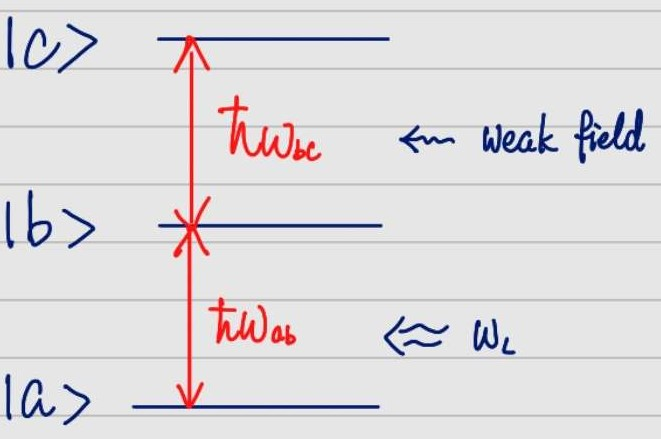
\includegraphics[scale=0.36]{542HW6/1}\\
Figure 1. The three-level atom.
\end{center}

The use of the weak field is mainly to probe the transition frequencies, here we focus on the effect of the intense field with photon frequency $\omega_L$ have on the system. We consider the energy states of the whole system. We label the states of the atom as $a,b,c$ and the number of the photon in the field as $N$. If the intense field and the atom are uncoupled, $|c,N\rangle$, $|a,N+1\rangle$, and $|b,N\rangle$ are three eigenstate of the system. While when the intense field and the atom are coupled, which is the case when the intense field is turned on the drive the atom, $|a,N+1\rangle$ and $b,N\rangle$ are no longer eigenstate, and the dressed states $|I(N)\rangle$ and $|II(N)\rangle$ which are superposition of $|a,N+1\rangle$ and $|b,N\rangle$, as shown in Figure 2, become the eigenstate of the system. \\

\begin{center}
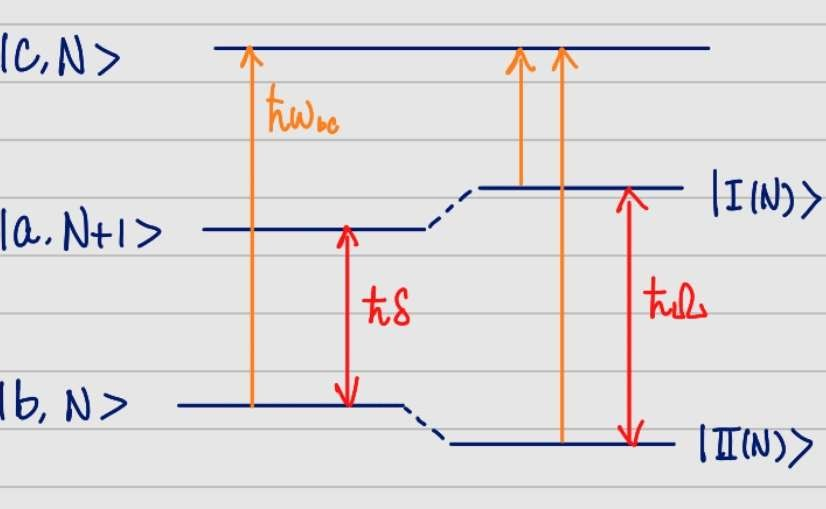
\includegraphics[scale=0.36]{542HW6/2}\\
Figure 2. The dressed-states of the three-level atom. 
\end{center}

The transition with frequency close to $\omega_{bc}$ can be probe by the weak field.
Since both $|I(N)\rangle$ and $|II(N)\rangle$ contain admixtures of
$|b, N\rangle$, the two transitions labeled by the orange arrow in Figure 2, $|I(N)\rangle \to |C,N\rangle$ and $|II(N)\rangle \to |2,N\rangle$ are allowed for the probe field. The absorption spectrum of this probe field is a single line when the intense field is off, now it becomes a doublet, known as the Autler-Townes doublet, when the intense field is on.\\

It remains to find the position of the doublet. The full Hamiltonian reads
\begin{align*}
H = H_{\text{A}} + H_{\text{F}} + H_{\text{int}}\,,
\end{align*}
where $H_{\text{A}}$ and $H_{\text{F}}$ are the Hamiltonian of the atom (with $|a\rangle$ and $|b\rangle$ states only) and field, respectively, and $H_{\text{int}}$ is the interaction Hamiltonian when the intense field is turned on. Here the state $|a,N+1\rangle$ and $|b,N\rangle$ are separated by
\begin{align*}
(N+1)\hbar \omega_L - \hbar \omega_L - \hbar \omega_{ab} = \hbar (\omega_L - \omega_{ab}) \coloneqq \hbar \delta\,,
\end{align*}
where $\delta=\omega_L - \omega_{ab}$ is the detuning. Here we let $\Omega_0$ denote the (real) Rabi frequency of the intense field, and denote
\begin{align*}
\Omega = \sqrt{\delta^2 + \Omega_0^2}\,.
\end{align*}
In particular, here we have the coupling term
\begin{align*}
\langle b, N | H_{\text{int}} | a, N+1\rangle = \hbar \Omega/2\,.
\end{align*}
Following the analysis as in the textbook, as the full Hamiltonian is of a form similar to that in the semiclassical dressed state analysis, it is not hard to see that the difference between between the dressed states is $\hbar \Omega$, and the resonances of the doublet thus occur at $\omega_{34}\pm \Omega/2$. 


\chapter{}
Following the notations from Berman, with 
\begin{align*}
|II_n\rangle = \cos(\theta_n) |2,n-1\rangle + \sin(\theta_n) |1,n\rangle\,,\qquad
|I_n\rangle = \cos(\theta_n) |1,n\rangle - \sin(\theta_n) |2,n-1\rangle
\end{align*}
being the eigenkets of the Jaynes-Cummings Hamiltonian. Denote $\Omega_ n =\sqrt{|2g_n|^2 + \delta^2}$. The energy diagram for the first few dressed-state manifolds of the system is given by the following.
\begin{center}
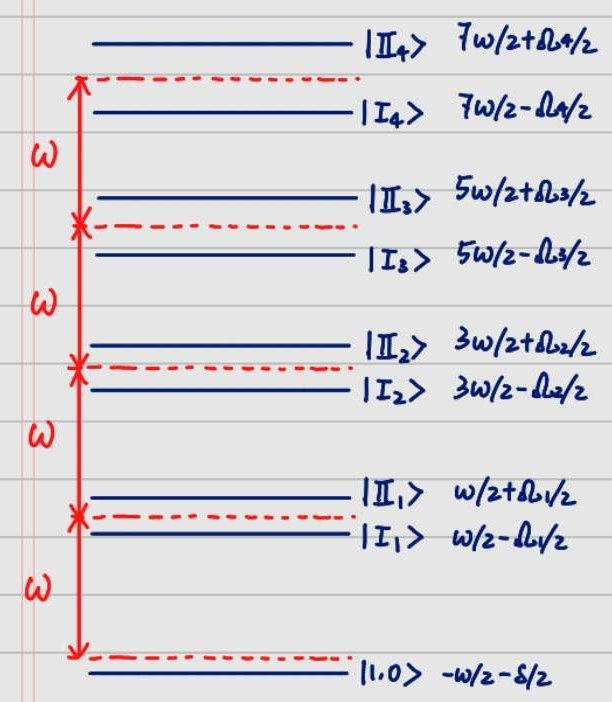
\includegraphics[scale=0.39]{542HW6/3}
\end{center}


\chapter{}
\textbf{(a)} According to Eq.\,(4.120), for atom initially in the excited state, $C_e = 1$ and $C_g = 0$, thus 
\begin{align*}
|\psi(t) \rangle 
&= \sum_{n=0}^\infty \left(C_n \cos(\lambda t\sqrt{n+1}) \right)|e\rangle |n\rangle+ \left(-i C_{n}\sin(\lambda t\sqrt{n+1}) \right)|g\rangle |n+1\rangle \\
&= \sum_{n=0}^\infty K_{e,n}|e\rangle |n\rangle+ K_{g, n}|g\rangle |n+1\rangle \\
\end{align*}
where we have abbreviated
\begin{align*}
K_{e,n} \coloneqq C_n \cos(\lambda t\sqrt{n+1}) \,,\qquad
K_{g,n} \coloneqq
-i C_{n}\sin(\lambda t\sqrt{n+1})\,.
\end{align*}
According to the problem, with $\alpha = \sqrt{30}$, we have
\begin{align*}
C_n = e^{-|\alpha|^2/2}\frac{\alpha^n}{\sqrt{n!}}\,.
\end{align*}
The density operator is given by
\begin{align*}
\hat{\rho} =  |\psi(t)\rangle \langle \psi(t)|\,,
\end{align*}
thus now we compute
\begin{align*}
\text{tr}_A(\hat{\rho}) 
&= 
\langle e |\hat{\rho}|e\rangle + \langle g| \hat{\rho}|g\rangle 
=
\sum_{n=0}^\infty\sum_{m=0}^\infty K_{e,n}K_{e,m}^* | n\rangle\langle m | + K_{g,n}K_{g,m}^* |n+1\rangle \langle m+1|\,.
\end{align*}
Thus we cam compute
\begin{align*}
S &= 1 - \text{tr}(\hat{\rho}_f^2) 
= 1 - \sum_{n=0}^\infty \langle n |\hat{\rho}_f^2|n\rangle\\
&= 1 - \sum_{n=0}^\infty \sum_{m=0}^\infty\langle n |\hat{\rho}_f | m \rangle \langle m |\hat{\rho}_f | n\rangle\\
&= 1- \sum_{n=0}^\infty\sum_{m=0}^\infty |\langle n |\hat{\rho}_f|m \rangle |^2\\
&=1 - \sum_{n=0}^\infty\sum_{m=0}^\infty \left|K_{g,n-1}^*K_{g,m-1} + K_{e,n}^* K_{e,m} \right|^2\\
&= 1- \sum_{n=0}^\infty\sum_{m=0}^\infty \left|
C_{n-1} \sin(\lambda t\sqrt{n})C_{m-1} \sin(\lambda t\sqrt{m})+C_n \cos(\lambda t \sqrt{n+1})C_m \cos(\lambda t \sqrt{n+1})
\right|^2\\
&= 1- \sum_{n=0}^\infty\sum_{m=0}^\infty |C_{n}C_m|^2\left|
\frac{\sqrt{nm}}{|\alpha|^{2}} \sin(\lambda t\sqrt{n}) \sin(\lambda t\sqrt{m})+\cos(\lambda t \sqrt{n+1}) \cos(\lambda t \sqrt{n+1})
\right|^2\\
&= 1- \sum_{n=0}^\infty\sum_{m=0}^\infty \frac{e^{-2|\alpha|^2}|\alpha|^{2(n+m)}}{n!m!} \left|
\frac{\sqrt{nm}}{|\alpha|^{2}} \sin(\lambda t\sqrt{n}) \sin(\lambda t\sqrt{m})+\cos(\lambda t \sqrt{n+1}) \cos(\lambda t \sqrt{n+1})
\right|^2\,,
\end{align*}
with $\alpha = \sqrt{30}$ in this case. \\
\begin{center}
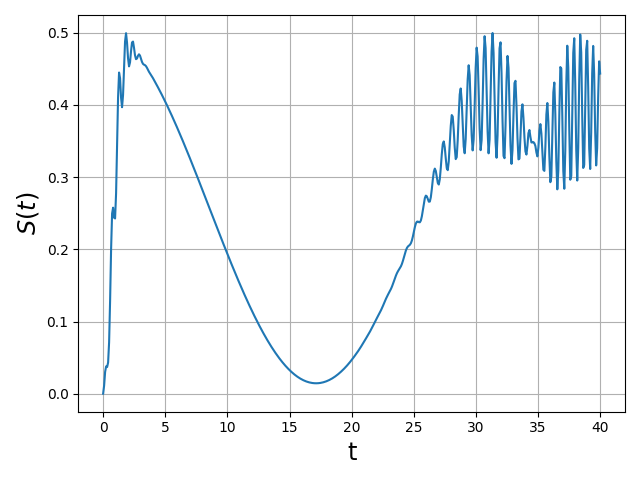
\includegraphics[scale=0.59]{542HW6/S(t)}
\end{center}
In the figure, $\lambda = 1$ and $\alpha = \sqrt{30}$. We recognize that the quantity $S(t)$ has the same trend as the von Neumann entropy of the system. When $t \sim 17$, which is a point where the atom and field are nearly in pure states and the von Neumann entropy of the system reaches a minimum as analyzed in Section 4.10 in the text, we see that $S(t)$ also reaches its minimum. That is there exists a point between the initial collapse of the
Rabi oscillations and the first revival where the system become least entangled and atom and field are nearly in pure states. 


\textbf{(b)} Here we compute the Q function
\begin{align*}
Q(\beta) &= \frac{1}{\pi}
\langle \beta | \hat{\rho}_f |\beta \rangle 
= \frac{e^{-|\beta|^2}}{\pi}\sum_n \sum_m \frac{(\beta^*)^n\beta^m}{\sqrt{n!m!}} \langle n |\hat{\rho}_f |m\rangle
\\
&= \frac{e^{-|\beta|^2}}{\pi} 
\sum_{m=0}^\infty\sum_{n=0}^\infty \frac{(\beta^*)^{n}\beta^m }{m!n!} 
C_nC_m^*
\left(
\frac{\sqrt{nm}}{|\alpha|^{2}} \sin(\lambda t\sqrt{n}) \sin(\lambda t\sqrt{m})+\cos(\lambda t \sqrt{n+1}) \cos(\lambda t \sqrt{n+1})
 \right)\\
&= \frac{e^{-|\beta|^2-|\alpha|^2}}{\pi} 
\sum_{m=0}^\infty\sum_{n=0}^\infty \frac{(\alpha\beta^*)^{n}(\alpha^*\beta)^m }{m!n!} 
\left(
\frac{\sqrt{nm}}{|\alpha|^{2}} \sin(\lambda t\sqrt{n}) \sin(\lambda t\sqrt{m})+\cos(\lambda t \sqrt{n+1}) \cos(\lambda t \sqrt{n+1})
 \right)\,,
\end{align*}
with $\alpha = \sqrt{30}$ in this case. Here $Q(\beta)$ verses time are plotted.  
\begin{center}
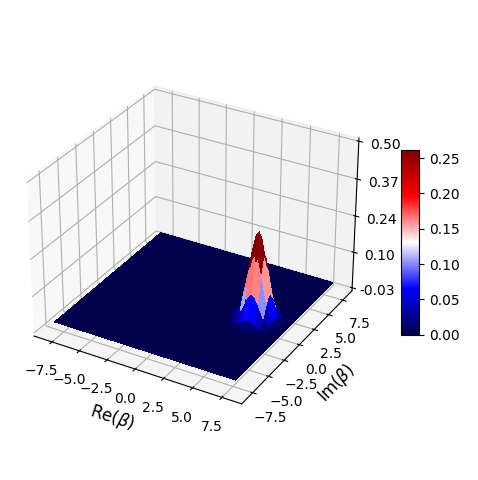
\includegraphics[scale=0.4]{542HW6/Q(0)}
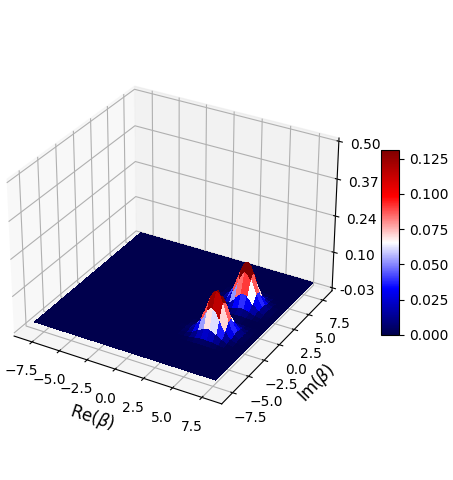
\includegraphics[scale=0.4]{542HW6/Q(5)}
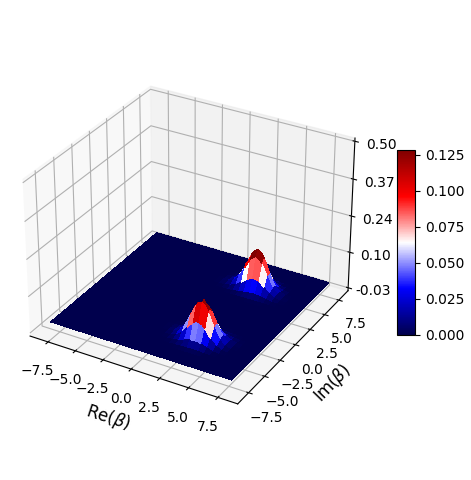
\includegraphics[scale=0.4]{542HW6/Q(10)}\\
$t=0$ \qquad\qquad\qquad\qquad\qquad $t=5$ \qquad\qquad\qquad\qquad\qquad $t=10$\\
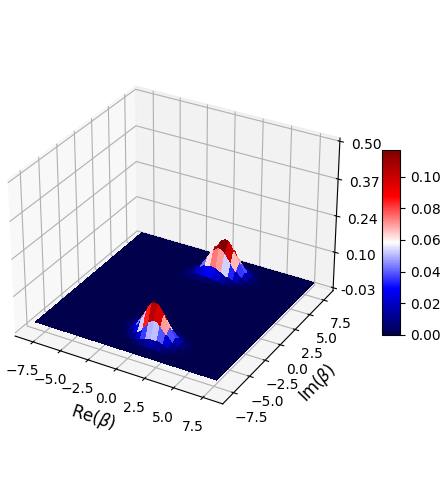
\includegraphics[scale=0.4]{542HW6/Q(15)}
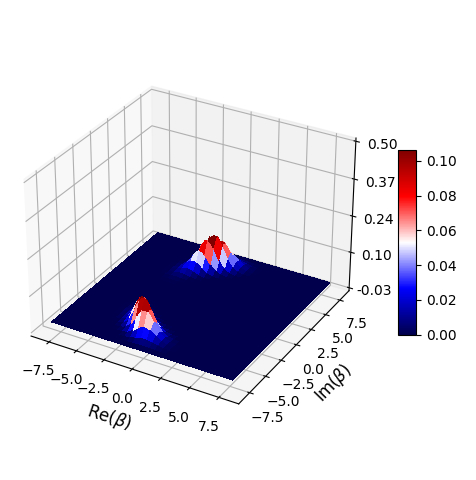
\includegraphics[scale=0.4]{542HW6/Q(20)}
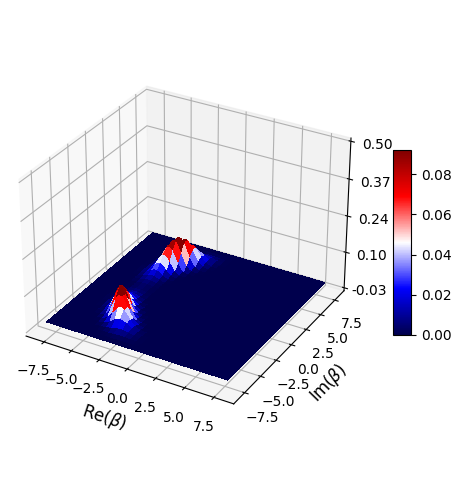
\includegraphics[scale=0.4]{542HW6/Q(25)}\\
$t=15$ \qquad\qquad\qquad\qquad\qquad $t=20$ \qquad\qquad\qquad\qquad\qquad $t=25$\\
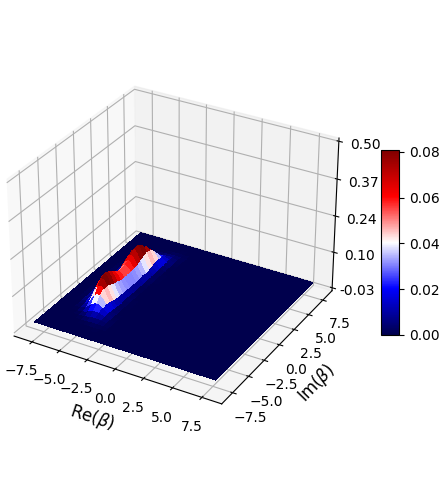
\includegraphics[scale=0.4]{542HW6/Q(30)}
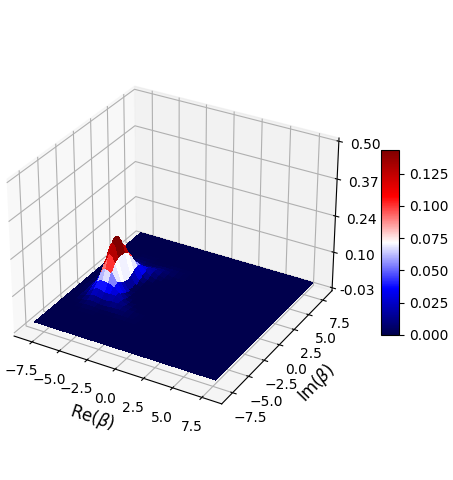
\includegraphics[scale=0.4]{542HW6/Q(35)}
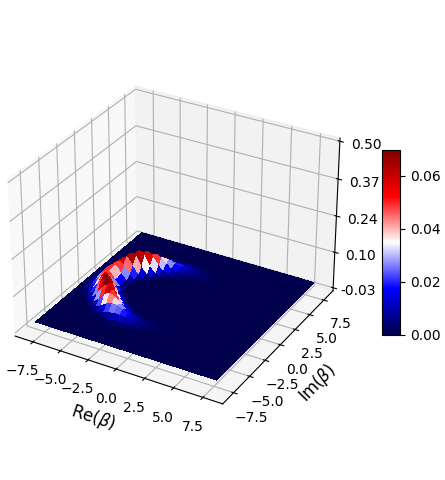
\includegraphics[scale=0.4]{542HW6/Q(40)}
$t=30$ \qquad\qquad\qquad\qquad\qquad $t=35$ \qquad\qquad\qquad\qquad\qquad $t=40$\\
\end{center}

\end{document}



